% The two split protocols (Ch. 3/4).
\documentclass[12pt,border=2pt]{standalone}
\usepackage[T1]{fontenc}\usepackage{newtxtext}
\usepackage{tikz}\usetikzlibrary{positioning,arrows.meta,calc}
\tikzset{
  box/.style={draw, rounded corners=2pt, align=center, font=\small, minimum height=10mm, text width=27mm, fill=white, line width=0.5pt},
  data/.style={box, fill=blue!10, draw=blue!55},
  proc/.style={box, fill=orange!12, draw=orange!70!black!70},
  res/.style={box, fill=green!12, draw=green!45!black!60},
  arr/.style={-{Latex[length=2mm]}, thick, draw=blue!35!black!55}}
\begin{document}
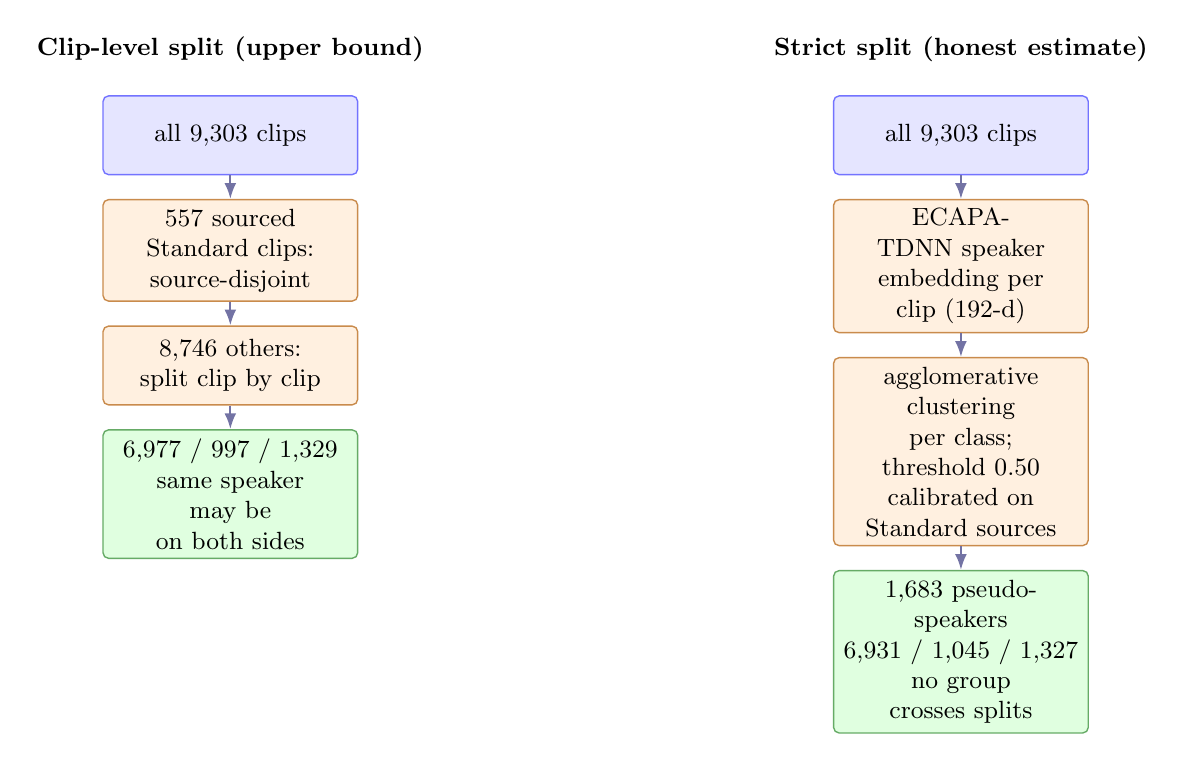
\begin{tikzpicture}[node distance=3mm and 8mm, box/.append style={text width=30mm}]
  \node[font=\small\bfseries] (t1) {Clip-level split (upper bound)};
  \node[data, below=of t1] (a1) {all 9,303 clips};
  \node[proc, below=of a1] (a2) {557 sourced Standard clips:\\source-disjoint};
  \node[proc, below=of a2] (a3) {8,746 others:\\split clip by clip};
  \node[res, below=of a3] (a4) {6,977 / 997 / 1,329\\same speaker may be\\on both sides};
  \draw[arr] (a1) -- (a2); \draw[arr] (a2) -- (a3); \draw[arr] (a3) -- (a4);
  \node[font=\small\bfseries, right=42mm of t1] (t2) {Strict split (honest estimate)};
  \node[data, below=of t2] (b1) {all 9,303 clips};
  \node[proc, below=of b1] (b2) {ECAPA-TDNN speaker\\embedding per clip (192-d)};
  \node[proc, below=of b2] (b3) {agglomerative clustering\\per class; threshold 0.50\\calibrated on Standard sources};
  \node[res, below=of b3] (b4) {1,683 pseudo-speakers\\6,931 / 1,045 / 1,327\\no group crosses splits};
  \draw[arr] (b1) -- (b2); \draw[arr] (b2) -- (b3); \draw[arr] (b3) -- (b4);
\end{tikzpicture}
\end{document}
